%%%%%%%%%%%%%%%%%%%%%%%%%%%%%%%%%%%%%%%%%%%%%%%%%%%
%% P3: Phenomenology of Particle Physics                         
%%
%% Author:  André Rubbia                   		 
%%
%% Figure 27.21 recision measurements of the Weinberg angle.
%%
%% This work is licensed under the Creative Commons Attribution 4.0 International License. 
%% To view a copy of this license, visit http://creativecommons.org/licenses/by/4.0/ or 
%% send a letter to Creative Commons, PO Box 1866, Mountain View, CA 94042, USA.
%%
%%%%%%%%%%%%%%%%%%%%%%%%%%%%%%%%%%%%%%%%%%%%%%%%%%%

\documentclass[a4paper,10pt]{article}

\usepackage[T1]{fontenc}
\usepackage[utf8]{inputenc}
\usepackage{lmodern}
\usepackage[labelfont=bf]{caption}
\usepackage{upgreek}

\usepackage{tikz}
\usepackage{pgfplots}
\pgfplotsset{compat=1.17}
\usepgfplotslibrary{ternary}
\usepgfplotslibrary{fillbetween}
\usepgfplotslibrary{external}

\def\d{\mathrm{d}}
\setlength{\oddsidemargin}{-1.0cm}
\setlength{\evensidemargin}{-1.0cm}
\setlength{\textheight}{25cm}
\setlength{\textwidth}{18cm}

\pgfkeys{/pgf/number format/.cd,1000 sep={}}

\begin{document}

%%%%%%%%%%%%%%%%   FIGURE  %%%%%%%%%%%%%%%%%%%%%%%%%%%%%%
\begin{figure}[htb]
 	\centering
		\begin{tikzpicture}[scale=1]
%
% sin2theta_W
%
\begin{axis}[
    xbar,
    width=10cm,
    height=7cm,
    title={Weinberg mixing angle},
    xlabel={$\sin^2\theta_{eff}$},
    symbolic y coords={ybot,average,$Q^{had}_{FB}$,$A^{0,c}_{FB}$,$A^{0,b}_{FB}$,
    $A_{LR}$,Asymmetry in $P_\tau$,$A^{0,l}_{FB}$,ytop},
    ytick=data,
    ymin=ybot,ymax=ytop,
    xmin=0.23, xmax=0.234,
    legend pos=north east,
x tick label style={
        /pgf/number format/.cd,
            fixed,
            fixed zerofill,
            precision=3,
        /tikz/.cd
    }
    ]
\addplot[
    color=blue,only marks,
    mark=*,
        error bars/.cd,
    x dir=both, x explicit
    ]
    coordinates {
   (0.23220,$A^{0,c}_{FB}$)+-(0.00081,0)
   (0.23221,$A^{0,b}_{FB}$)+-(0.00029,0)
   (0.23098,$A_{LR}$)+-(0.00026,0)
   (0.23159,Asymmetry in $P_\tau$)+-(0.00041,0)
   (0.23099,$A^{0,l}_{FB}$)+-(0.00053,0)
   (0.2324,$Q^{had}_{FB}$)+-(0.0012,0)
   (0.23153,average)+-(0.00016,0)
};
   \draw[gray,fill,fill opacity=0.2] (axis cs:0.23137,ybot) rectangle (axis cs:0.23169,ytop);
\end{axis}
\end{tikzpicture}
	\caption{Precision measurements of the Weinberg angle. Data from
	S.~Schael {\em et~al.}, ``{Precision electroweak measurements on the $Z$
  resonance},'' {\em Phys. Rept.}, vol.~427, pp.~257--454, 2006.}
\end{figure}
%
%%%%%%%%%%%%%%%%   END FIGURE  %%%%%%%%%%%%%%%%%%%%%%%%%%%%%%
%


\end{document}
